\documentclass{article}
\usepackage{cmap}
\usepackage[utf8]{inputenc}
\usepackage[english,ukrainian]{babel}
\usepackage{graphicx}
\usepackage{geometry}
\usepackage{listings}
\usepackage{float}
\usepackage{amsmath}
\geometry{
	a4paper,
	left=20mm,
	right=20mm,
	top=15mm,
	bottom=15mm,
}
\lstset{
	language=c,
	tabsize=4,
	keepspaces,
	breaklines=true,
	showstringspaces=false,
}
\graphicspath{ {./pictures} }
\setlength{\parindent}{4em}

\newcommand\subject{Програмування в Інтернет}
\newcommand\lecturer{асистент кафедри ПЗ \\ Степанов Д.С.}
\newcommand\teacher{доцент кафедри ПЗ \\ Грицай О.Д.}
\newcommand\mygroup{ПЗ-22}
\newcommand\lab{6}
\newcommand\theme{Основні типи та функції доступу до БД MongoDB}
\newcommand\purpose{Засвоїти елементи створення, модифікації, читання та занесення даних з таблиць БД засобами Node.js}

\begin{document}
\begin{normalsize}
\begin{titlepage}
	\thispagestyle{empty}
	\begin{center}
		\textbf{МІНІСТЕРСТВО ОСВІТИ І НАУКИ УКРАЇНИ\\
			НАЦІОНАЛЬНИЙ УНІВЕРСИТЕТ "ЛЬВІВСЬКА ПОЛІТЕХНІКА"}
	\end{center}
	\begin{flushright}
		\textbf{ІКНІ}\\
		Кафедра \textbf{ПЗ}
	\end{flushright}
	\vspace{200pt}
	\begin{center}
		\textbf{ЗВІТ}\\
		\vspace{10pt}
		до лабораторної роботи № \lab\\
		\textbf{на тему}: “\textit{\theme}”\\
		\textbf{з дисципліни}: “\subject”
	\end{center}
	\vspace{112pt}
	\begin{flushright}
		
		\textbf{Лектор}:\\
		\lecturer\\
		\vspace{28pt}
		\textbf{Виконав}:\\
		
		студент групи \mygroup\\
		Коваленко Д.М.\\
		\vspace{28pt}
		\textbf{Прийняв}:\\
		
		\teacher\\
		
		\vspace{28pt}
		«\rule{1cm}{0.15mm}» \rule{1.5cm}{0.15mm} 2023 р.\\
		$\sum$ = \rule{1cm}{0.15mm}……………\\
		
	\end{flushright}
	\vspace{\fill}
	\begin{center}
		\textbf{Львів — 2023}
	\end{center}
\end{titlepage}
	
\begin{description}
	\item[Тема.] \theme.
	\item[Мета.] \purpose.
\end{description}

\section*{Індивідуальне завдання}

\begin{figure}[H]
	\centering
	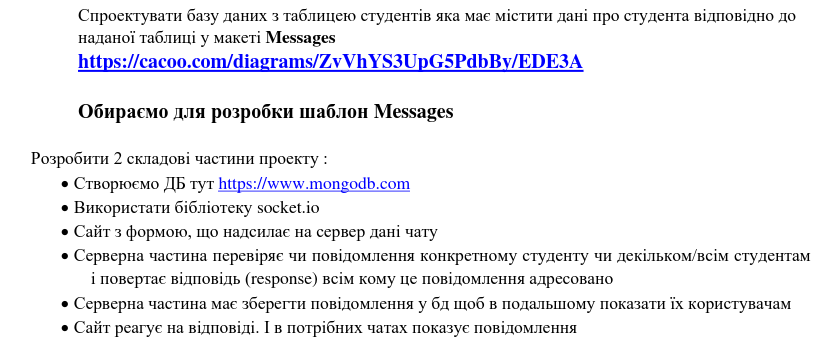
\includegraphics[width=\textwidth]{v}
\end{figure}


\section*{Теоретичні відомості}
Node.js - це опенсорсне кросплатформове середовище виконання для JavaScript, яке
працює на серверах.
Платформа Node.js побудована на базі JavaScript двигун V8 від Google, який
використовується в браузері Google Chrome. Ця платформа в основному використовується
для створення веб-серверів, проте сфера її застосування цим не обмежується.
Однією з основних привабливих особливостей Node.js є швидкість. JavaScript-код,
що виконується в середовищі Node.js, може бути вдвічі швидше, ніж код, написаний
компілюваними мовами, на кшталт C або Java, і на порядки швидше за інтерпретовані
мови на кшталт Python або Ruby.

У традиційних мовах програмування (C, Java, Python, PHP) всі інструкції за
замовчуванням є блокуючими, якщо тільки розробник явно не подбає про асинхронне
виконання коду. В результаті якщо, наприклад, у такому середовищі, зробити мережевий
запит для завантаження якогось JSON-коду, виконання потоку, з якого зроблений запит,
буде припинено доти, доки не завершиться отримання та обробка відповіді.

JavaScript значно спрощує написання асинхронного та неблокуючого коду з
використанням єдиного потоку, функцій зворотного виклику (коллбеків) та підходу до
розробки, що базується на подіях. Щоразу, коли нам потрібно виконати важку операцію,
ми передаємо відповідному механізму коллбек, який буде викликаний одразу після
завершення цієї операції. В результаті, щоб програма продовжила роботу, чекати
результатів виконання подібних операцій не потрібно.

Подібний механізм виник у браузерах. Ми не можемо дозволити собі чекати, скажімо,
закінчення виконання AJAX-запиту, не маючи при цьому можливості реагувати на дії
користувача, наприклад на клацання по кнопках. Для того, щоб користувачам було зручно
працювати з веб-сторінками, все, і завантаження даних з мережі, і обробка натискання на
кнопки має відбуватися одночасно, в режимі реального часу.
Якщо ви створювали колись обробник події натискання на кнопку, то ви вже
користувалися методиками асинхронного програмування.

Завдяки простоті та зручності роботи з менеджером пакетів для Node.js, який
називається npm, екосистема Node.js розвивається. Зараз у реєстрі npm є понад
півмільйона опенсорсних пакетів, які може вільно використовувати будь-який Node.js-
розробник.

\section*{Хід виконання}
\begin{lstlisting}
const Room = require('./models/room');
const { Message } = require('./models/message');
const User = require('./models/user');

const socketIO = require('socket.io');

function init(server) {
	const io = socketIO(server, {
		cors: {
			origin: '*',
			methods: ['GET', 'POST'],
		},
	});
	
	io.on('connection', (socket) => {
		socket.on('getUnreadRooms', async (username) => {
			try {
				const user = await User.findOne({ username }).populate('unreadRoomIds').exec();
				if (!user) {
					return;
				}
				const unreadRooms = await Room.find({
					_id: { $in: user.unreadRoomIds },
					users: { $in: [username] }
				}).lean().exec();
				
				io.to(socket.id).emit('unreadRooms', unreadRooms);
			} catch (err) {
				console.error(err);
			}
		});
		
		socket.on('setRoomAsRead', async (roomId, username) => {
			try {
				const user = await User.findOne({ username });
				
				const room = await Room.findOne({ _id: roomId, users: { $in: [username] } });
				
				console.log('Setting room as read!');
				console.log(username, roomId);
				
				const updatedUser = await User.findByIdAndUpdate(user._id, { $pull: { unreadRoomIds: room._id } }, { new: true });
			} catch (err) {
				console.error(err);
			}
		});
		
		socket.on('getOldMessages', async (roomId) => {
			try {
				const room = await Room.findById(roomId).populate({ path: 'messages', populate: { path: 'senderId' }, options: { strictPopulate: false } }).exec();
				console.log('Getting old messages for room!');
				console.log(room);
				const messages = room.messages.map(message => {
					return {
						_id: message._id,
						senderId: message.senderId._id,
						author: message.senderId.username,
						isReadByToId: message.isReadByToId,
						content: message.content,
						createdAt: message.createdAt,
						updatedAt: message.updatedAt,
					}
				});
				io.to(roomId).emit('oldMessages', messages);
			} catch (err) {
				console.error(err);
			}
		});
		
		socket.on('newMessage', async (roomId, username, messageContent) => {
			const sender = await User.findOne({ username });
			if (!sender) {
				return console.error(`Sender ${username} not found`);
			}
			
			const message = new Message({ content: messageContent, senderId: sender._id });
			console.log('Got new message!');
			console.log(message);
			console.log(sender);
			
			try {
				const savedMessage = await message.save();
				const room = await Room.findById(roomId);
				room.messages.push(savedMessage._id);
				
				const connectedUsernames = Object.keys(io.sockets.adapter.rooms[roomId]?.sockets || {}).filter(socketId => socketId !== socket.id);
				const connectedUsers = await User.find({ username: { $in: connectedUsernames } });
				console.log(connectedUsers.map(u => u.username));
				
				const users = await User.find({ username: { $in: room.users } });
				const senderIndex = users.findIndex(user => user.username === sender.username);
				if (senderIndex !== -1) {
					users.splice(senderIndex, 1);
				}
				const nonConnectedUsers = users.filter(user => !connectedUsernames.includes(user.username));
				for (const user of nonConnectedUsers) {
					user.unreadRoomIds.addToSet(room._id);
					await user.save();
					console.log('Setting unread room for user!');
					console.log(user.username, room.name);
				}
				
				await room.save();
				io.to(roomId).emit('newMessage', sender.username, messageContent);
			} catch (error) {
				console.error(error);
			}
		});
		
		socket.on('joinRoom', (roomId) => {
			console.log(`Socket ${socket.id} joining room ${roomId}`);
			socket.join(roomId);
		});
		
		socket.on('leaveRoom', (roomId) => {
			console.log(`Socket ${socket.id} leaving room ${roomId}`);
			socket.leave(roomId);
		});
	});
	
	return io;
}

module.exports = init;
\end{lstlisting}

\section*{Результат роботи}
\begin{figure}[H]
	\centering
	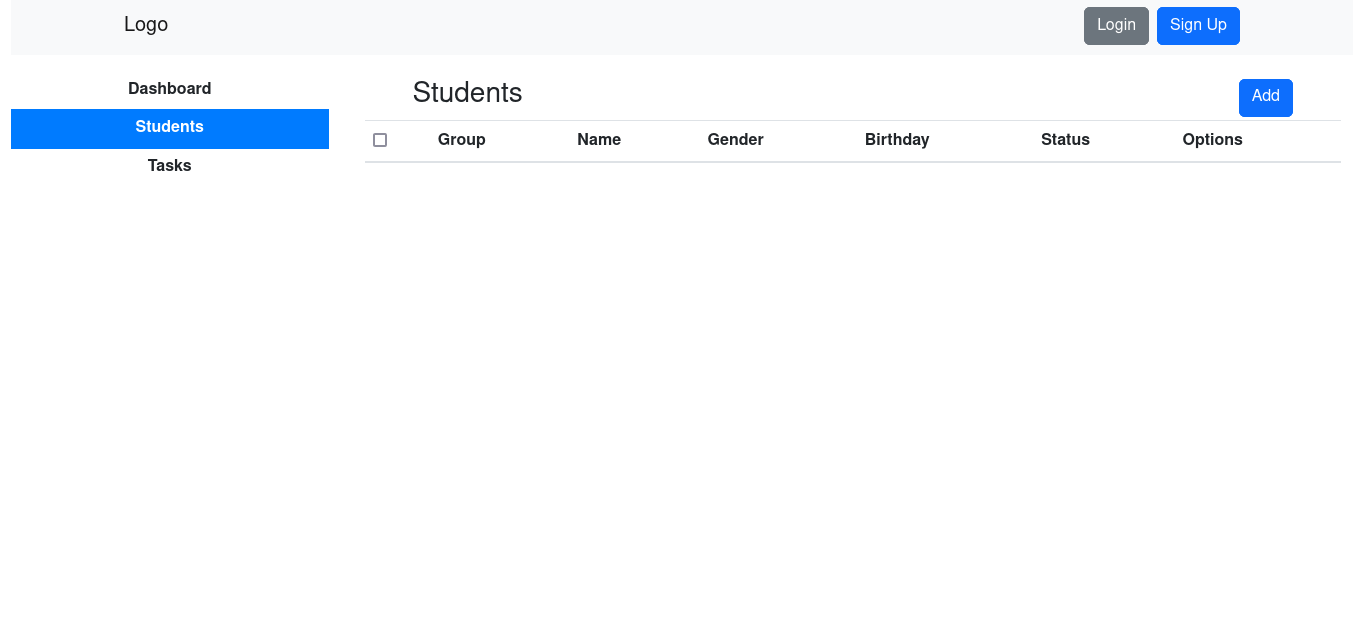
\includegraphics[width=\textwidth]{1}
\end{figure}

\begin{figure}[H]
	\centering
	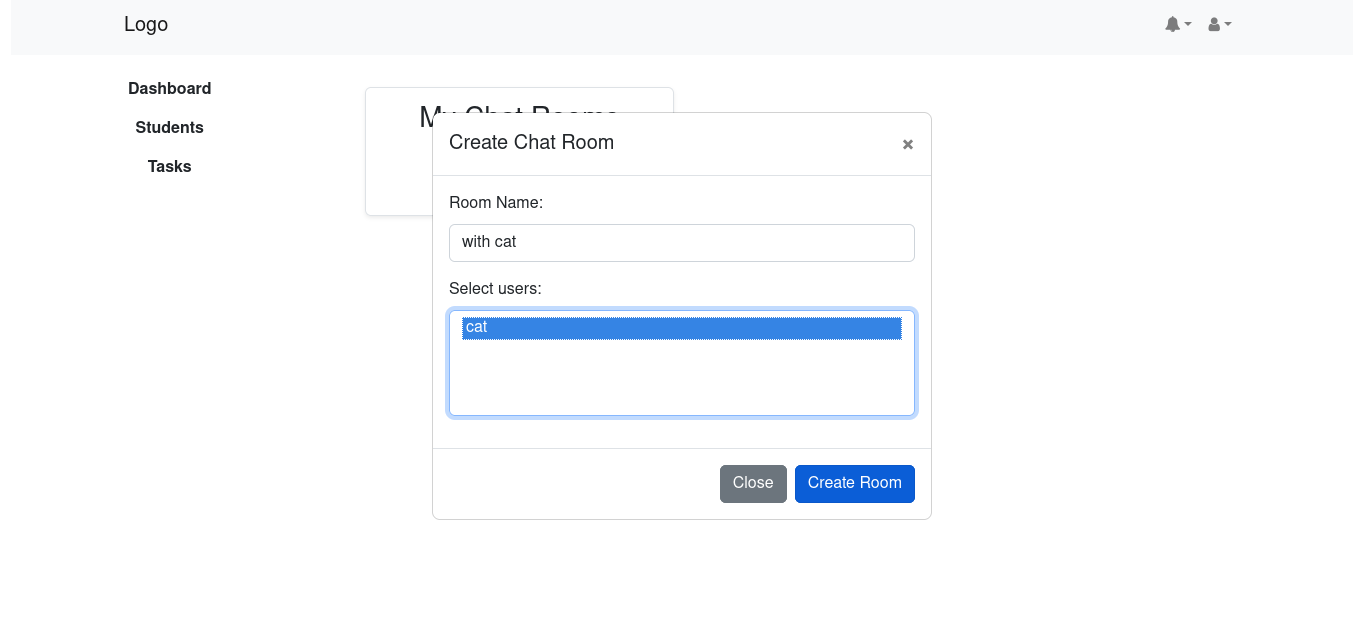
\includegraphics[width=\textwidth]{2}
\end{figure}

\begin{figure}[H]
	\centering
	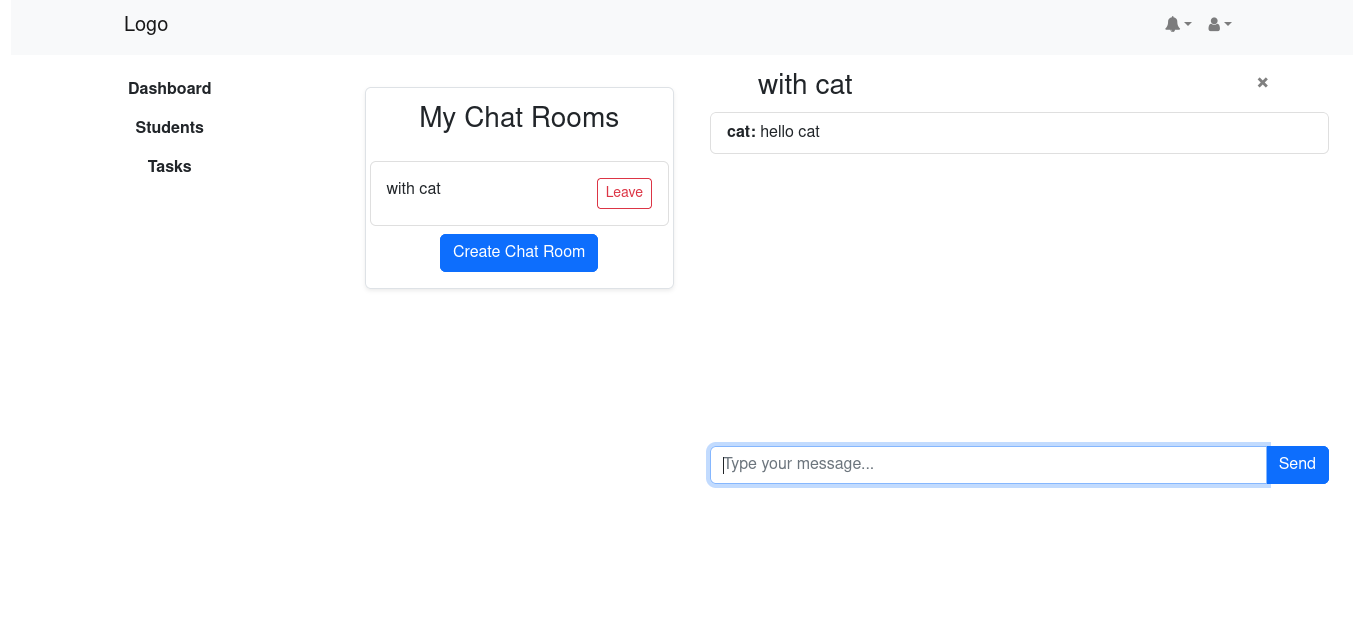
\includegraphics[width=\textwidth]{3}
\end{figure}

\begin{figure}[H]
	\centering
	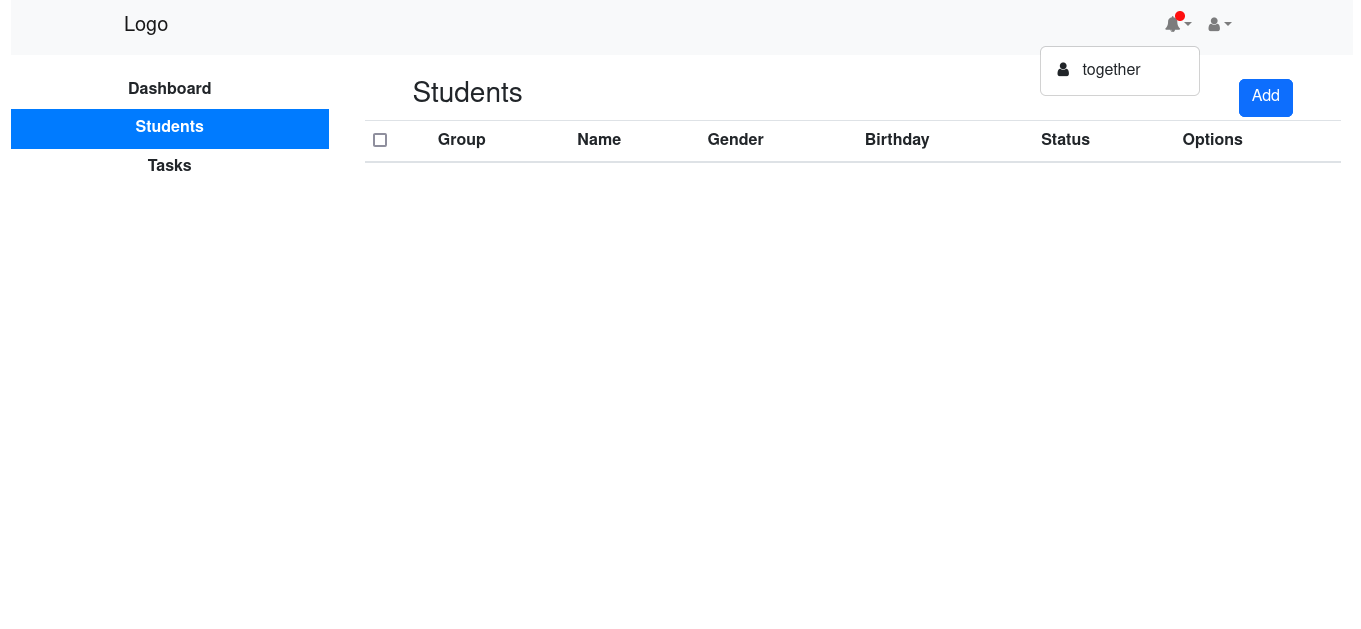
\includegraphics[width=\textwidth]{4}
\end{figure}

\begin{figure}[H]
	\centering
	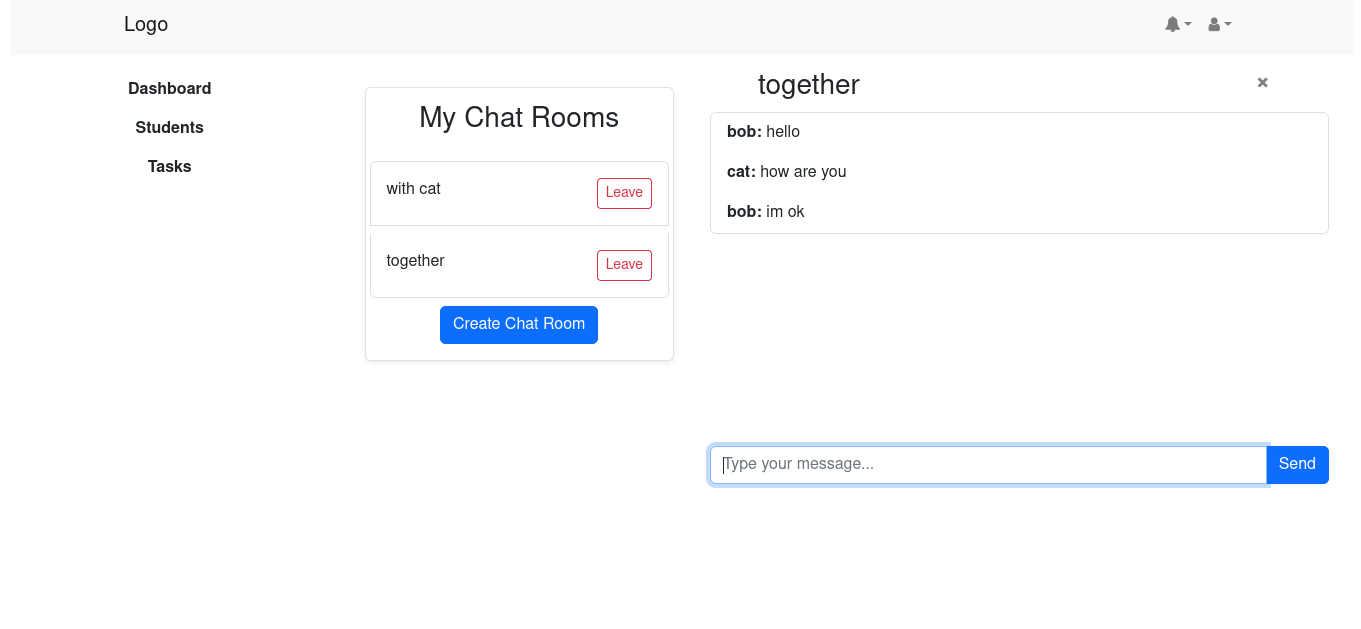
\includegraphics[width=\textwidth]{5}
\end{figure}

\section*{Висновки}
Під час виконання лабораторної роботи я засвоїв елементи створення, модифікації, читання та занесення даних з
таблиць БД засобами Node.js
	    
\end{normalsize}
\end{document}
